\documentclass[report.tex]{subfiles}

\begin{document}

\chapter{Applications to MCMC Algorithms}
\label{chapter-mcmc-applications}

In this chapter we show how the current PDMP based MCMC algorithms can be
efficiently implemented by using our framework, namely, the Bouncy Particle
Sampler \cite{bouchard2015bouncy} and the Zig-Zag process \cite{bierkens2016zig}.
We further show how our analysis framework can assist in solving the current
research problems.

\section{The Bouncy Particle Sampler}

\subsection{The Global Scheme}

Suppose we want to generate samples from some probability distribution
$\pi$ over $\mathbb{R}^{d}$ which we can evaluate only up to a positive normalising constant, that is:
$$
\pi(x) \propto \gamma(x).
$$
Further, let
$$
U(x) = -\log \gamma(x)
$$
and call $U$ the \textit{energy function}.

Now consider a $\mathbb{R}^{2d} = (X, V)$ state space, where the first $d$ variables represent
position of a particle, while the last $d$ variables represent velocity (just like
in the toy PDMP example introduced in Section~\ref{pdmp-toy-example-section}).
Define the \textit{intensity function} $\lambda$ on such state space as:
$$
\lambda(x, v) = \langle \nabla U(x), v \rangle^{+}
$$
and define the \textit{reflection operation}:
$$
R(x)v
= \left(I_{d} - 2\frac{\nabla U(x) (\nabla U(x))^{T}}{\lVert \nabla U(x) \rVert^{2}}\right)v
= v - 2 \frac{\langle \nabla U(x), v\rangle}{\lVert \nabla U(x) \rVert^{2}}\nabla U(x)
$$
where $\lVert \cdot \rVert$ is the $L^{2}$ norm.
The reflection operator reflects the velocity $v$ on the hyperplane tangent to the
energy function gradient at the given position $x$.

Further, let $\lambda_{\text{ref}} > 0$ be the \textit{refresh rate} and let
$\psi$ be a standard normal multivariate $d$-dimensional probability density.
The Bouncy Particle Sampler is then a PDMP, given by the following generator:
\begin{align*}
  \mathcal{A}f(x, v) &= \langle \nabla_{x} f(x, v), v\rangle \\
                     &+ \lambda(x, y)(f(x, R(x)v) - f(x, v)) \\
                     &+ \lambda_{\text{ref}} \myint{}{}{(f(x, v') - f(x, v))\psi(v')}{v'}.
\end{align*}
The first term is the linear flow, the second term corresponds to reflecting the velocity,
while the last term corresponds to simply resampling the velocity.
See \cite{peters2012rejection, bouchard2015bouncy} for justification of such procedure.
Every point in the resulting trajectory generated by our PDMP is a sample from
the invariant distribution $\pi$.
The law of large numbers becomes integrating instead of summation.
See Figure~\ref{image-bps-refresh-rates} for some samples trajectories generated
with different refresh rate parameters.


\begin{figure}
  \captionsetup{skip=0.75cm}
  \centering
  \begin{subfigure}{.25\textwidth}
    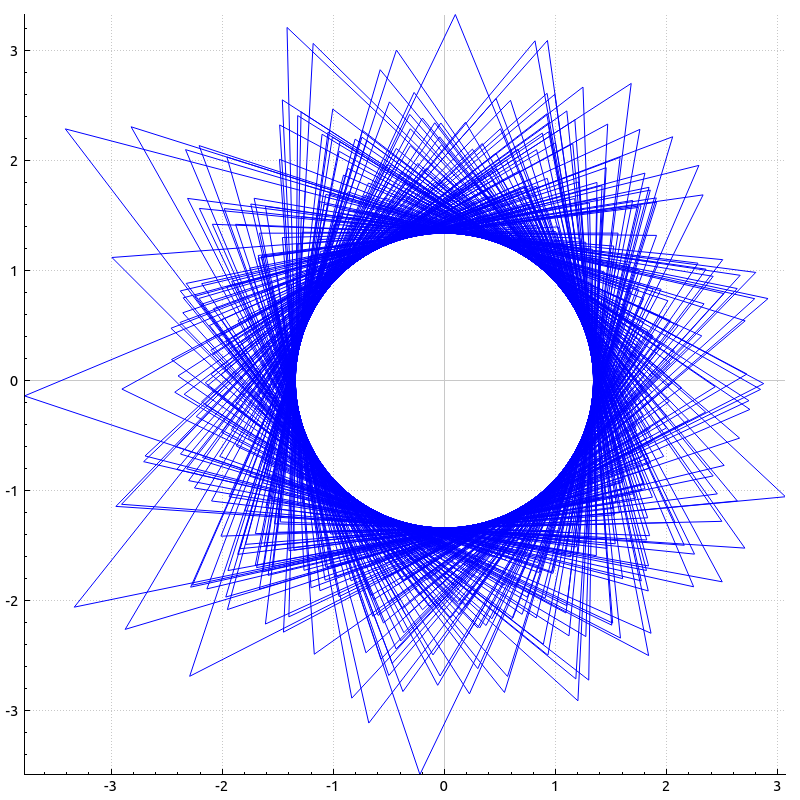
\includegraphics[width=\textwidth]{img/bps_ref_0_0001}
    \caption*{$\lambda_{\text{ref}} = 10^{-4}$}
  \end{subfigure}
  \begin{subfigure}{.25\textwidth}
    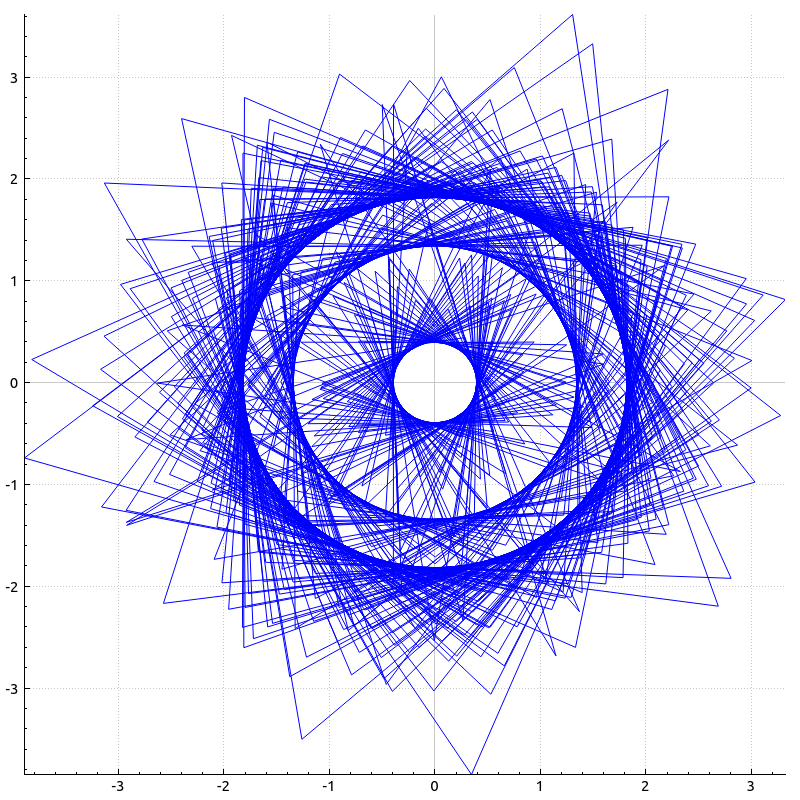
\includegraphics[width=\textwidth]{img/bps_ref_0_001}
    \caption*{$\lambda_{\text{ref}} = 10^{-3}$}
  \end{subfigure}
  \begin{subfigure}{.25\textwidth}
    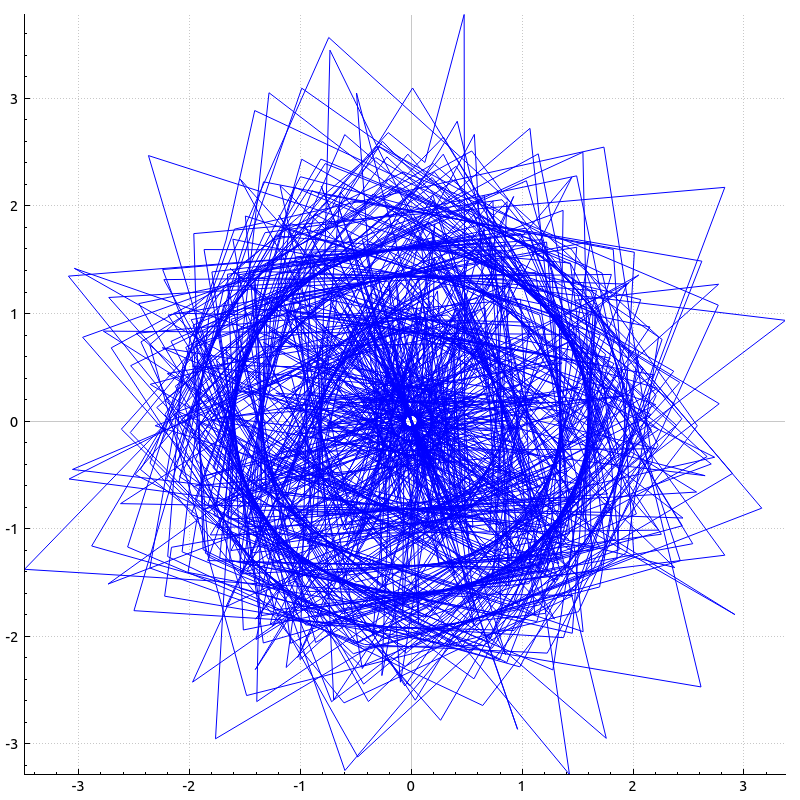
\includegraphics[width=\textwidth]{img/bps_ref_0_01}
    \caption*{$\lambda_{\text{ref}} = 10^{-2}$}
  \end{subfigure}
  \begin{subfigure}{.25\textwidth}
    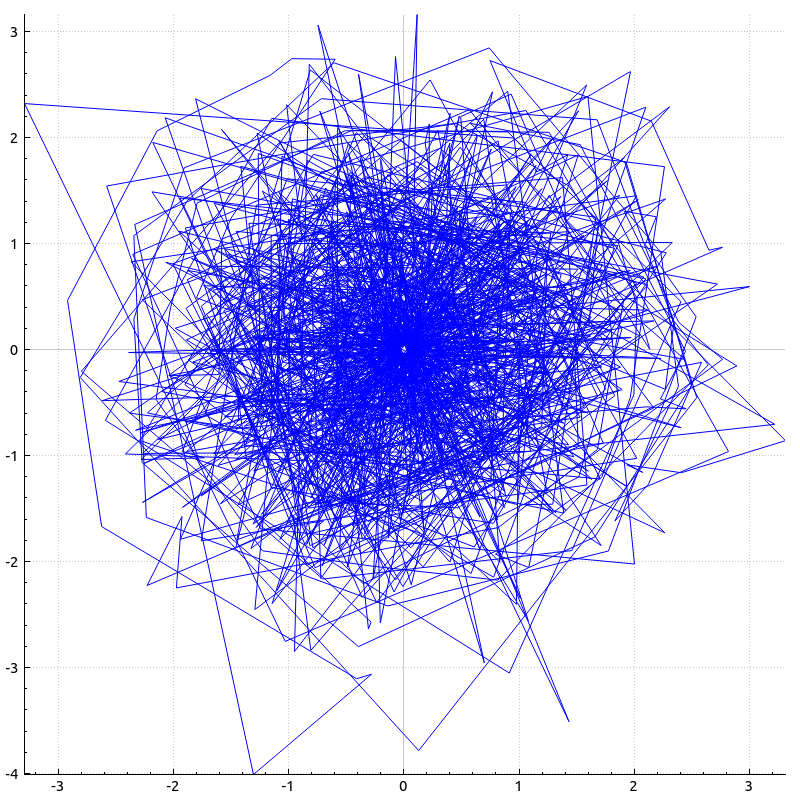
\includegraphics[width=\textwidth]{img/bps_ref_0_1}
    \caption*{$\lambda_{\text{ref}} = 10^{-1}$}
  \end{subfigure}
  \begin{subfigure}{.25\textwidth}
    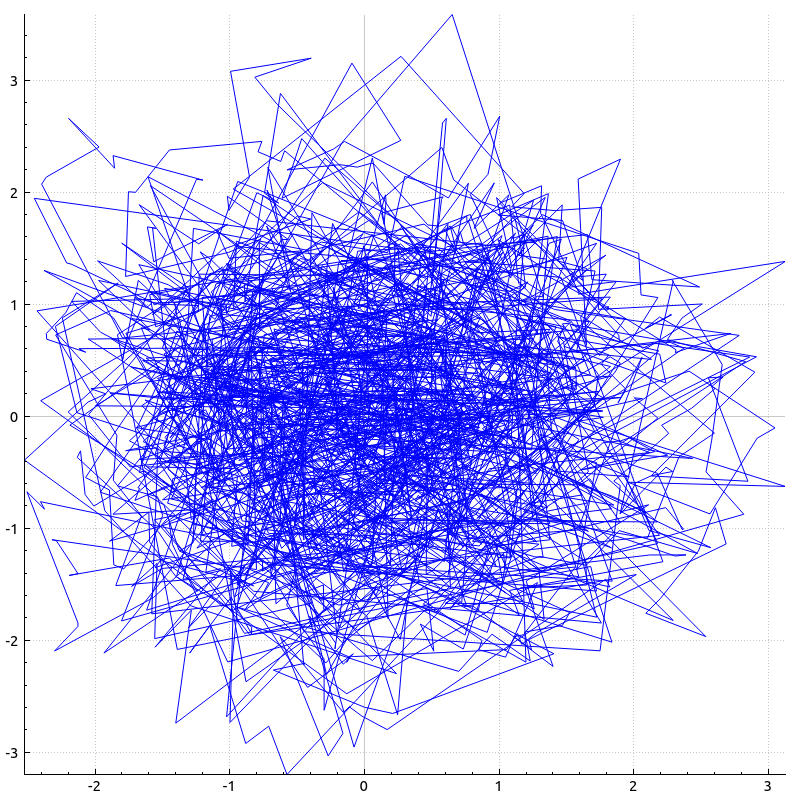
\includegraphics[width=\textwidth]{img/bps_ref_1}
    \caption*{$\lambda_{\text{ref}} = 1$}
  \end{subfigure}
  \begin{subfigure}{.25\textwidth}
    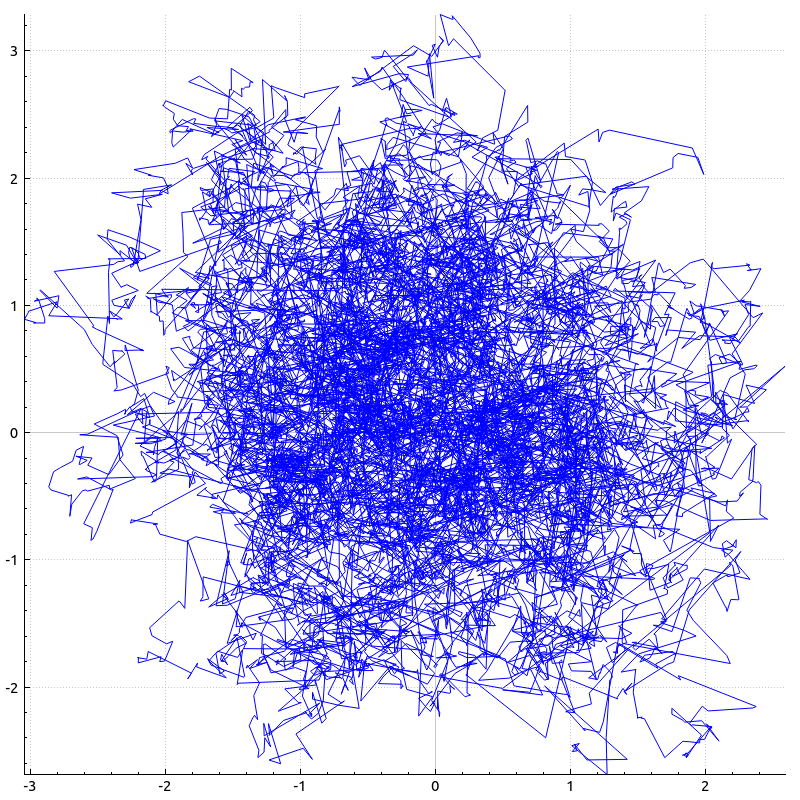
\includegraphics[width=\textwidth]{img/bps_ref_10}
    \caption*{$\lambda_{\text{ref}} = 10$}
  \end{subfigure}
  \begin{subfigure}{.25\textwidth}
    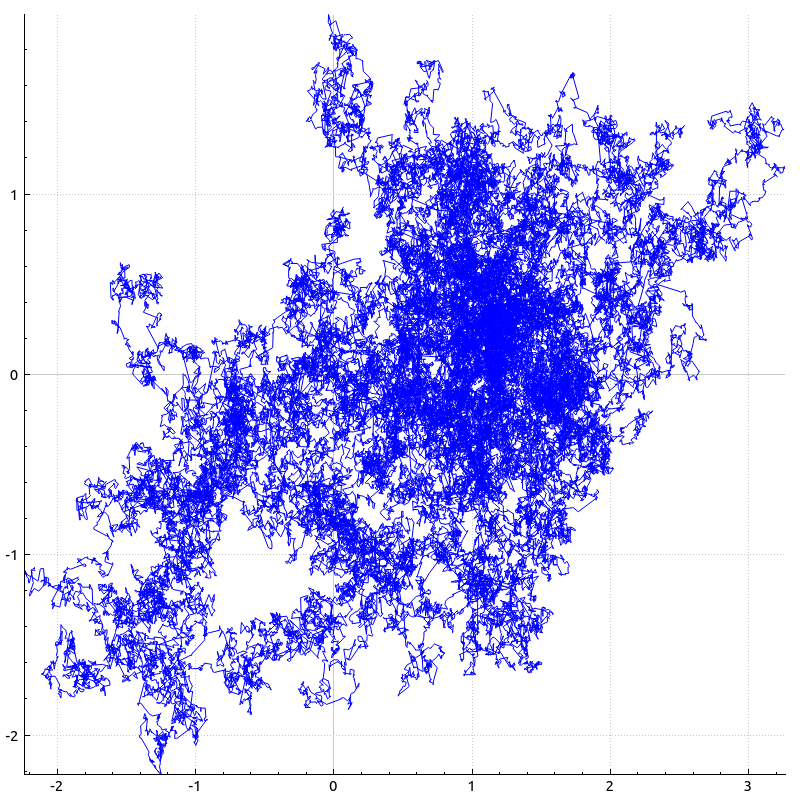
\includegraphics[width=\textwidth]{img/bps_ref_100}
    \caption*{$\lambda_{\text{ref}} = 10^{2}$}
  \end{subfigure}
  \begin{subfigure}{.25\textwidth}
    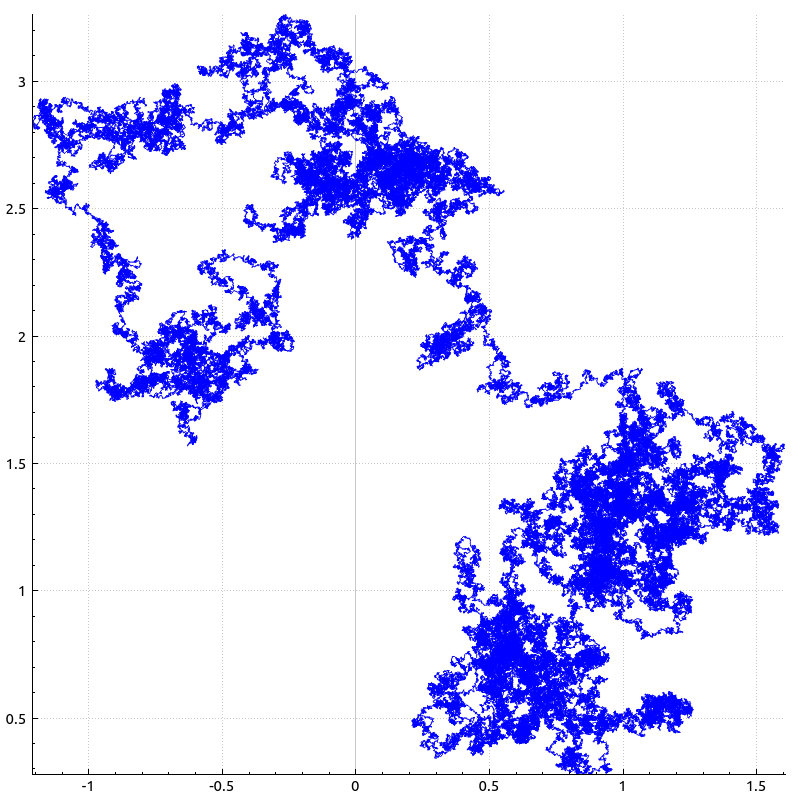
\includegraphics[width=\textwidth]{img/bps_ref_1000}
    \caption*{$\lambda_{\text{ref}} = 10^{3}$}
  \end{subfigure}

  \caption{The role of the refresh rate parameter in the Bouncy Particle Sampler.
           In each image, a trajectory path of the BPS is plotted, where
           the target distribution is 2-dimensional standard normal.
           Both too small and too large values of $\lambda_{\text{ref}}$ lead to
           difficulties in exploration of the state space. Indeed, it was shown
           in \citet{bouchard2015bouncy} that with $\lambda_{\text{ref}} = 0$ the
           resulting Markov process need not be ergodic.
           See examples/path\_plotting/ in the project's GitHub repository for
           reproducing these plots by using our analysis framework.}
  \label{image-bps-refresh-rates}
\end{figure}

\subsection{The Local Scheme}

Now supose that
$$
\gamma(x) = \prod_{f \in F} \gamma_{f}(x_{f}).
$$
Then the energy function writes as a sum of (local) energies.
Consequently, we can associate a (local) intensity factor $\lambda_{f}$ and a (local) reflection
operator $R_{f}$ with each factor $f \in F$ in the same way as we did in the global BPS scheme above.
The local Bouncy Particle Sampler is then a PDMP with infinitesimal generator given by:
\begin{align*}
  \mathcal{A}h(x, v) &= \langle \nabla_{x} h(x, v), v\rangle \\
                     &+ \sum_{f \in F} \lambda_{f}(x, y)(h(x, R_{f}(x)v) - h(x, v)) \\
                     &+ \lambda_{\text{ref}} \myint{}{}{(h(x, v') - h(x, v))\psi(v')}{v'}.
\end{align*}
See \cite{bouchard2015bouncy} for full details. This local BPS scheme is extremely useful
in scenarios where we have a lot of factors and the dependencies between them are very
sparse.

\subsection{Implementation}
The good news is that there is not really much that we need to implement.
Indeed, in Chapter~\ref{pdmps-implementation} we have already efficiently implemented
processes of such type.
The Poisson process simulation is model dependent and thus will have to be specified by the user.
So the only thing we need to do is implement the reflection operator, which is easy to do.

To take away the burden of gradient calculations and basic probability densities definitions
we have added the Stan mathematics library developed by \citet{carpenter2015stan} to our project, which was
built for almost identical use case as ours (Hamiltonian Monte Carlo simulations).

Finally, we provided a builder class for creating the BPS algorithm, which simply takes
our specificaly designed probability distribution class as input for adding factors to the generator.
The probability distribution objects encapsulate how to simulate Poisson process jump times
associated to them, while the BPS builder class in addition adds reflection kernels as well
as the refreshment kernel.
See project's code repository for full implementation details.
Listing~\ref{bps-builder-code} a code example of using the builder and our probability
distribution classes.

\begin{lstfloat}
\caption{Example usage of the BPS algorithm within our framework.}
\label{bps-builder-code}
\begin{lstlisting}
// Create a standard normal 2-dimensional distribution object.
RealMatrix covariances(2, 2);
covariances << 1, 0,
               0, 1;
RealVector mean(2);
mean << 0, 0;
mcmc::GaussianDistribution gaussianDistribution(mean, covariances);

// Create a PDMP simulating the BPS algorithm.
pdmp::mcmc::BpsBuilder bpsBuilder(2);
bpsBuilder.addFactor(
  {0,1}, // Specify the model variables on which this factor acts.
  gaussianDistribution);
// Add more factors if needed...
auto pdmp = bpsBuilder.build();

// Now select a PDMP runner and output processors from the analysis
// framework to perform arbitrary actions as needed.
\end{lstlisting}
\end{lstfloat}

\section{The Zig-Zag Process}

The Zig-Zag process is similar to the BPS, except that instead of performing
velocity reflections, during each event time ir multiplies one velocity component
by $-1$ (flips that component). See \citet{bierkens2016zig} for details.
This essentially means that we can reuse almost all the code used to construct
the BPS PDMPs -- we only need to change the reflection kernel with the flipping
kernel. See the project's code repository for implementation details.
See Figure~\ref{zig-zag-path} for an example trajectory generated by the Zig-Zag process.
See Figure~\ref{zig-zag-vs-bps} for how our framework can be used to compare the BPS and
the Zig-Zag process.

\begin{SCfigure}
  \centering
  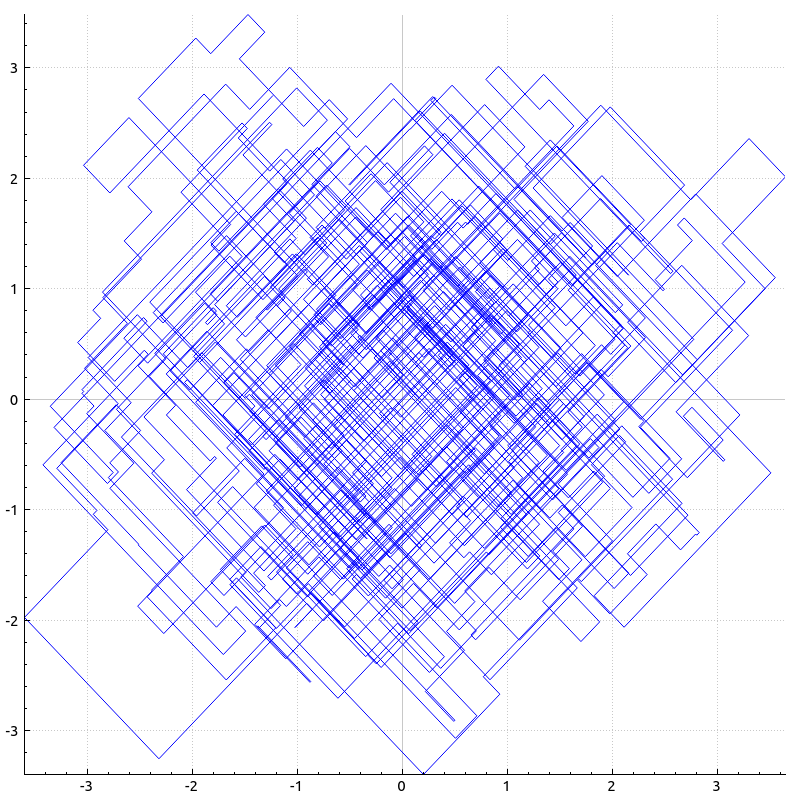
\includegraphics[width=.45\textwidth]{img/zig_zag_path}
  \caption{A sample path generated by the Zig-Zag process on the bivariate
     standard normal distribution as its target.
     Note that at the event times only one velocity component is changed.
     See /examples/path\_plotting/ in the project's GitHub repository for code.}
  \label{zig-zag-path}
\end{SCfigure}

\begin{SCfigure}
  \centering
  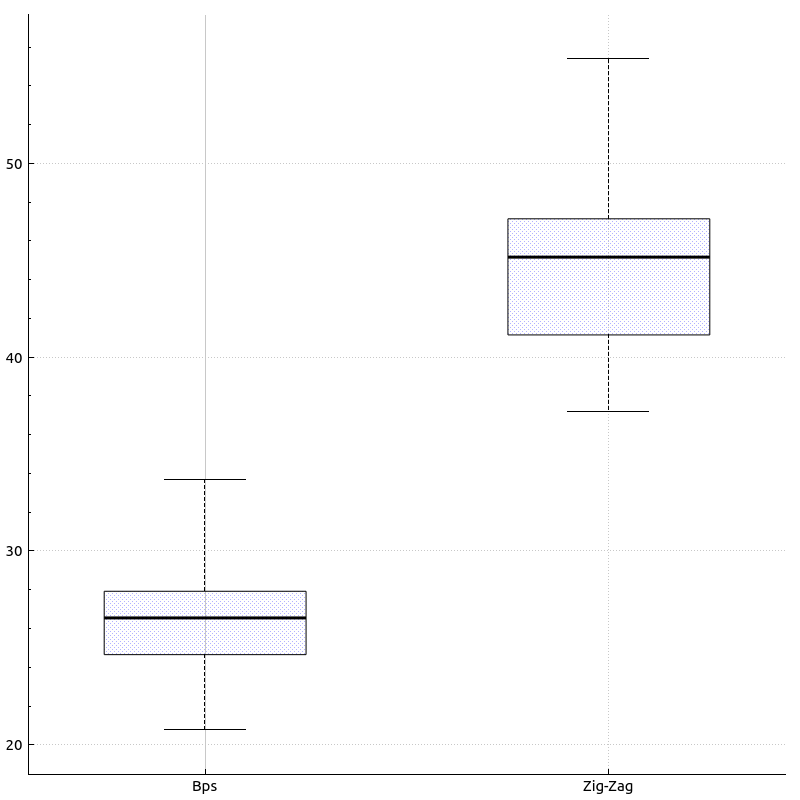
\includegraphics[width=.45\textwidth]{img/asymptotic_var}
  \caption{Comparison of asymptotic variances (see Appendix~\ref{mcmc-output-analysis})
           of the BPS and the Zig-Zag process on a two-dimensional standard Gaussian target, where
           the function we integrate along the path is the squared $L^{2}$-norm.
           Each algorithm was run 42 times to generate the box plot.
           We have used our analysis framework's to run many processes in parallel.
           See /examples/compare\_bps\_zig\_zag/ directory in the project's GitHub page
           for the code used to run this experiment. Note that no parameters were tuned
           for either of the algorithms, this example is merely meant to demonstrate
           the capabilities of our framework. Listing~\ref{bps-vs-zig-zag-code} shows the
           sketch of code used efficiently generate such graphs.}
  \label{zig-zag-vs-bps}
\end{SCfigure}

\begin{lstfloat}
\caption{Sketch code for comparing different algorithms just as we did in Figure~\ref{zig-zag-vs-bps}}
\label{bps-vs-zig-zag-code}
\begin{lstlisting}
double getBpsAsymptoticVariance() {
  // Create a new BPS process and use our output analysis framework
  // to run it and calculate the asymptotic variance.
  ...
  return calculatedAsymptoticVarianceForThisRun;
}

double getZigZagAsymptoticVariance() {
  // Same as above, but for the Zig-Zag process.
  ...
  return calculatedAsymptoticVarianceForThisRun;
}

int main() {
  ParallelWorkers<double> bpsWorkers, zigZagWorkers;
  // Launch 40 BPS processes on 8 cores.
  auto bpsAsymptoticVariances = bpsWorkers.executeTasksInParallel(
    getBpsAsymptoticVariance, 40, 8);
  // Launch 40 Zig-Zag processes on 8 cores.
  auto zigZagAsymptoticVariances = zigZagWorkers.executeTasksInParallel(
    getZigZagAsymptoticVariance, 40, 8);

  plotBoxPlot(
    {bpsAsymptoticVariances, zigZagAsymptoticVariances},
    {"Bps", "Zig-Zag"});

  return 0;
}
\end{lstlisting}
\end{lstfloat}


\end{document}
